\documentclass[a4paper,10pt]{report}\input{../0.Préambule/Préambule_cours_prof}\input{0_Préambule_Algèbre}\begin{document}

\newpage
\setcounter{chapter}{4}
\hypertarget{Les nombres 3}{}
\chapter{Les nombres 3}

\section{Racine carrée d'un nombre}

\begin{dft}
$\sqrt{a}$ est le nombre positif qui a pour carré $a$.
\end{dft}

\medskip
\noindent $a$ est un carré, donc un nombre positif ; 

\noindent ainsi $\sqrt{-5}$ n'existe pas.
\medskip

\noindent Quelques valeurs exactes à connaître :

\vspace{-15mm}
\begin{flushright}
\renewcommand{\arraystretch}{1.5}
\begin{tabular}{|c|c|c|c|c|c|c|c|c|c|c|c|}\hline
$a$&0&1&4&9&16&25&36&49&64&81&100\\\hline
$\sqrt{a}$&0&1&2&3&4&5&6&7&8&9&10\\\hline
\end{tabular}
\end{flushright}

\vspace{-6mm}
\begin{rmq}
Tous les nombres $a$ figurant dans ce tableau sont des carrés parfaits. Plus généralement, on appellera carré parfait les nombres dont la racine carrée est un entier.

\medskip
\noindent Mais une racine carrée ne peut pas toujours s'écrire sous forme d'un entier, d'un décimal ou d'une fraction.

\noindent Par exemple, la seule écriture exacte de la racine carrée de 2 est $\sqrt{2}$. On dit que $\sqrt{2}$ est irrationnel.
\end{rmq}

\begin{demoe}
Proposition à démontrer : \og $\sqrt{2}$ est irrationnel \fg.

\medskip
On va démontrer cette proposition par l'absurde.

\smallskip
\noindent Supposons que $\sqrt{2}$ soit rationnel. Alors $\sqrt{2}$ est de la forme $\frac{a}{b}$, $a$ et $b$ deux entiers positifs et premiers entre eux. (la fraction $\frac{a}{b}$ ne peut plus être simplifiée)

\noindent On en déduit que : 
$$\sqrt{2} = \dfrac{a}{b}\quad \Longleftrightarrow \quad
\sqrt{2} {\color{cocours} \times b}= \dfrac{a}{b}{\color{cocours} \times b}\quad \Longleftrightarrow \quad
\sqrt{2} \times b = a\quad \Longleftrightarrow \quad
\left( \sqrt{2}\times b \right) {\color{cocours}^2} =  a {\color{cocours}^2}\quad \Longleftrightarrow \quad
\sqrt{2}^2 \times \left( b \right)^2 = a^2\quad \Longleftrightarrow \quad
2 \times b^{2} = a^2 $$
Puisque $a^2$ est pair, $a$ est pair donc $a=2p$ avec $p$ un entier positif
$$2 \times b^{2} = (2p)^2\quad \Longleftrightarrow \quad
2 \times b^{2} = 4p^2\quad \Longleftrightarrow \quad
b^{2} = 2p^2$$

\noindent On en déduit que $b^2$ est pair donc que $b$ est pair.

\medskip
\noindent Par conséquent, il est possible de simplifier la fraction $\frac{a}{b}$ par $2$, ce qui contredit l'hypothèse que $a$, $b$ sont premiers entre eux. 

\medskip
\noindent Puisque l'hypothèse \og $\sqrt{2}$ est rationnel \fg ~~ conduit à une contradiction, c'est le contraire qui est vrai, à savoir : 

\og $\sqrt{2}$ est irrationnel \fg.\hfill $\blacksquare$
\end{demoe}

\begin{prop}
Si $a$ et $b$ sont deux entiers naturels, alors $\sqrt{a} \times \sqrt{b} = \sqrt{a\times b}$
\end{prop}

\medskip
\begin{demoe}
Proposition à démontrer : $\sqrt{a} \times \sqrt{b} = \sqrt{a\times b}$

\begin{center}
$\sqrt{a\times b} ^2 \quad = \quad a\times b \quad = \quad \sqrt{a}^2 \times \sqrt{b}^2 \quad = \quad \left( \sqrt{a} \times \sqrt{b} \right) ^2 $
\end{center}

$\sqrt{a\times b}$ \quad et \quad $\sqrt{a} \times \sqrt{b}$ \quad étant positif, on peut en conclure que :
\[\sqrt{a} \times \sqrt{b} = \sqrt{a\times b}\]

\vspace{-8mm}
\hfill $\blacksquare$
\end{demoe}

\begin{meth}
Regroupements et simplifications d'écritures :

\begin{enumerate}
\item[•] on cherche à décomposer le nombre qui est sous le radical en un produit dont l'un des facteurs est un carré.
\begin{enumerate}
\item[-]$\sqrt{20} = \sqrt{4\times 5} = \sqrt{4} \times \sqrt{5} = 2\sqrt{5}$
\item[-]$\sqrt{32} = \sqrt{16\times 2} = \sqrt{16} \times \sqrt{2} = 4\sqrt{2}$
\item[-]$\sqrt{108} = \sqrt{36\times 3} = \sqrt{36} \times \sqrt{3} = 6\sqrt{3}$
\end{enumerate}
\item[•]dans un produit on cherche à associer les racines carrées d'un même nombre :
\begin{enumerate}
\item[-]$\sqrt{2}\times \sqrt{14} = \sqrt{2}\times \sqrt{2\times 7} = \sqrt{2}\times \sqrt{2}\times \sqrt{7} = \left(\sqrt{2}\right)^2 \times \sqrt{7} = 2 \sqrt{7}$
\item[-]$\sqrt{3}\times \sqrt{30} \times \sqrt{5}= \sqrt{3}\times \sqrt{3\times 5\times 2} \times \sqrt{5}= \sqrt{3}\times \sqrt{3}\times \sqrt{5} \times \sqrt{5}\times \sqrt{2}= \left(\sqrt{3}\right)^2 \times \left(\sqrt{5}\right)^2 \times \sqrt{2} = 3 \times 5 \times \sqrt{2} = 15\sqrt{2}$
\end{enumerate}
\item[•]on cherche à réduire les sommes en mettant les racines identiques en facteur :
\begin{enumerate}
\item[-]$3\sqrt{2}+5\sqrt{2} = (3+5)\times \sqrt{2} = 8\sqrt{2}$
\item[-]$3\sqrt{7}-2\sqrt{7} +\sqrt{7}= (3-2+1)\times \sqrt{7} = 2\sqrt{7}$
\end{enumerate}
\end{enumerate}
Ces calculs ont pour but d'obtenir un résultat dont l'écriture est la plus simple possible.
\end{meth}

%\begin{ex}
%$\sqrt{3} \times \sqrt{2} = \sqrt{3\times 2} = \sqrt{6} $
%\end{ex}

\begin{exec}
\hspace{0.5cm} \hypertarget{Ex_3_1_1}{} Exercice \ref{3_1_1} \hspace{0.5cm};
\hspace{0.5cm} \hypertarget{Ex_3_1_2}{} \ding{79} Exercice \ref{3_1_2} \hspace{0.5cm}
\end{exec}

\begin{rmq}
\begin{enumerate}
\item Ce résultat se généralise à tous les nombres positifs et pas uniquement aux entiers.
\item Si de plus $b \ne 0$, alors de même: 

\vspace{-7mm}
\[ \frac{\sqrt{a}}{\sqrt{b}}=\sqrt{\frac{a}{b}}. \]
\item Attention : en général $\sqrt{a} + \sqrt{b}$ N'EST PAS ÉGAL à $\sqrt{a + b}$
\quad($\sqrt{9} + \sqrt{16}= 3 + 4 = 7$ ; mais $\sqrt{9 + 16} = \sqrt{25} = 5$ )
\end{enumerate}
\end{rmq}

\begin{exec}
\hspace{0.4cm} \hypertarget{Ex_3_1_3}{} \phantom{\ding{79}} Exercice \ref{3_1_3} \hspace{0.4cm};
\hspace{0.4cm} \hypertarget{Ex_3_1_4}{} \ding{79} Exercice \ref{3_1_4} \hspace{0.4cm};
\hspace{0.4cm} \hypertarget{Ex_3_1_5}{} \phantom{\ding{79}} Exercice \ref{3_1_5} \hspace{0.5cm};
\hspace{0.4cm} \hypertarget{Ex_3_1_6}{} \ding{79} Exercice \ref{3_1_6} \hspace{0.4cm};
\hspace{0.4cm} \hypertarget{Ex_3_1_7}{} \ding{79} Exercice \ref{3_1_7} \hspace{0.4cm}
\end{exec}

\begin{prop}[Inégalité triangulaire]
Pour tout nombre strictement positif $a$ et $b$,  $\sqrt{a + b} < \sqrt{a} + \sqrt{b}$
\end{prop}

\begin{demoe}
Proposition à démontrer : $\sqrt{a + b} < \sqrt{a} + \sqrt{b}$
\begin{align*}
\left( \sqrt{a} + \sqrt{b} \right) ^2 \quad = \quad \left( \sqrt{a} + \sqrt{b} \right) \times \left( \sqrt{a} + \sqrt{b} \right) \quad &= \quad \sqrt{a}^2 + \sqrt{a}\sqrt{b} + \sqrt{b}\sqrt{a} + \sqrt{b}^2 \\
&> \sqrt{a}^2 + \sqrt{b}^2 \quad = \quad \quad a+b \quad = \quad \sqrt{a+b} ^2 
\end{align*}
$\sqrt{a+b}$ et $\sqrt{a} + \sqrt{b}$ étant positif, on peut en conclure que :
$\sqrt{a + b} < \sqrt{a} + \sqrt{b}$\hfill $\blacksquare$
\end{demoe}

\vspace{-3mm}
\section{Les nombres réels : $\mathbb{R}$}

\vspace{-3mm}
\begin{dft}
L'ensemble des nombres réels est l'ensemble de tous les nombres que nous utiliserons en classe de seconde.

\noindent L'ensemble des nombres réels est noté : $\mathbb{R}$.
\end{dft}

\medskip
L'ensemble des nombres réels peut être représenté, schématisé par une droite. 

\begin{center}
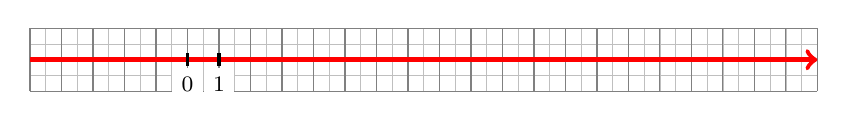
\begin{tikzpicture}[scale=0.4]
\def\xY{-5};
\def\yY{-1};
\def\xZ{20};
\def\yZ{1};
\coordinate (Y) at (\xY,\yY);
\coordinate (Z) at (\xZ,\yZ);
\draw[step=0.5cm, lightgray, very thin] (Y) grid (Z);
\draw[step=1cm, gray,thin] (Y) grid (Z);
\draw[ ->,line width=1.7pt,red] (\xY, 0) -- (\xZ, 0);
\foreach \x in {0,1}	\draw[very thick](\x,0.2cm)--(\x,-0.2cm) node[below,fill=white]{\footnotesize \x};
\end{tikzpicture}
\end{center}

\vspace{-3mm}
De même qu'en géométrie on s'intéresse à des morceaux de la droite, nous allons nous intéresser à des morceaux de l'ensemble des réels.
	
\noindent De façon plus terre à terre, dans la réalité (mathématiques appliquées) ou dans certaines situations ($\sqrt{x}$ et d'autres fonctions) nous seront amenés à utiliser des morceaux de l'ensemble des réels : des intervalles.

\begin{dft}
Un intervalle est un sous-ensemble (une partie) "sans trous" de l'ensemble des nombres réels $\mathbb{R}$.
\end{dft}

\subsection{Intervalles bornés}

Les intervalles bornés sont les ensembles qui contiennent tous les réels qui sont compris entre deux bornes (limites).

\begin{ex}

L'intervalle $[-2\ ;\ 13]$ (lisez \og fermé en $-2$ et fermé en $13$\fg{}) désigne l'ensemble des nombres réels $x$ compris entre $-2$ et $13$. Ce sont donc tous les nombres $x$ qui vérifient $ -2\leqslant x \leqslant 13 $

\noindent L'ensemble des nombres réels est représenté par une droite et l'intervalle $[-2\ ;\ 13]$ est alors représenté par un segment.

\vspace{-3mm}
\begin{center}
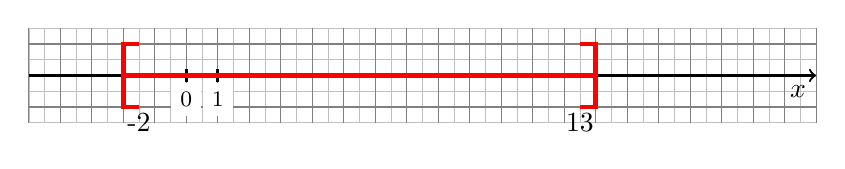
\begin{tikzpicture}[scale=0.4]
\def\xY{-5};
\def\yY{-1.5};
\def\xZ{20};
\def\yZ{1.5};
\coordinate (Y) at (\xY,\yY);
	\coordinate (Z) at (\xZ,\yZ);
	\draw[step=0.5cm, lightgray, very thin] (Y) grid (Z);
	\draw[step=1cm, gray,thin] (Y) grid (Z);
	\draw[ ->,thick] (\xY, 0) -- (\xZ, 0) node[below left]{$x$};
	\foreach \x in {0,1}	\draw[very thick](\x,0.2cm)--(\x,-0.2cm) node[below,fill=white]{\footnotesize \x};
	\def\xbornea{-2};
	\def\orientationa{1};
	\draw[line width=1.7pt,red] ({\xbornea+0.5*\orientationa},1)--(\xbornea,1)--(\xbornea,-1)--({\xbornea+0.5*\orientationa},-1);
	\draw(\xbornea+0.5,-1.5)node{\xbornea};
	\def\xborneb{13};
	\def\orientationb{1};
	\draw[line width=1.7pt,red] ({\xborneb-0.5*\orientationb},1)--(\xborneb,1)--(\xborneb,-1)--({\xborneb-0.5*\orientationb},-1);
	\draw(\xborneb-0.5,-1.5)node{\xborneb};
	\draw[line width=1.7pt,red](\xbornea,0)--(\xborneb,0);
	\end{tikzpicture}
	\end{center}
\end{ex}

Il arrive souvent qu'en cherchant à optimiser la taille des intervalles, il faille exclure les valeurs aux bornes. Ainsi pour désigner l'ensemble de tous les nombres compris entre $-2$ et $13$ mais pas $-2$ nous noterons: $]-2\ ;\ 13]$ (lisez \og ouvert en $-2$ et fermé en $13$\fg{}). 

\noindent Ce qui correspond à tous les nombres $x$ qui vérifient l'encadrement $ -2< x \leqslant 13$

	\begin{center}
	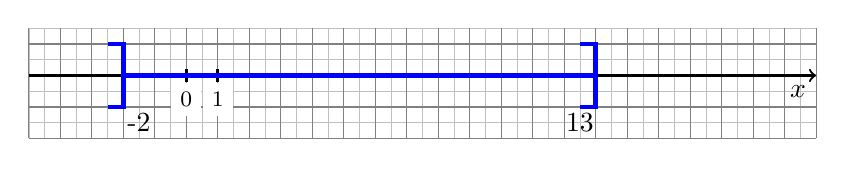
\begin{tikzpicture}[scale=0.4]
	\def\xY{-5};
	\def\yY{-2};
	\def\xZ{20};
	\def\yZ{1.5};
	\coordinate (Y) at (\xY,\yY);
	\coordinate (Z) at (\xZ,\yZ);
	\draw[step=0.5cm, lightgray, very thin] (Y) grid (Z);
	\draw[step=1cm, gray,thin] (Y) grid (Z);
	\draw[ ->,thick] (\xY, 0) -- (\xZ, 0) node[below left]{$x$};
	\foreach \x in {0,1}	\draw[very thick](\x,0.2cm)--(\x,-0.2cm) node[below,fill=white]{\footnotesize \x};
	\def\xbornea{-2};
	\def\orientationa{-1};
	\draw[line width=1.7pt,blue] ({\xbornea+0.5*\orientationa},1)--(\xbornea,1)--(\xbornea,-1)--({\xbornea+0.5*\orientationa},-1);
	\draw(\xbornea+0.5,-1.5)node{\xbornea};
	\def\xborneb{13};
	\def\orientationb{1};
	\draw[line width=1.7pt,blue] ({\xborneb-0.5*\orientationb},1)--(\xborneb,1)--(\xborneb,-1)--({\xborneb-0.5*\orientationb},-1);
	\draw(\xborneb-0.5,-1.5)node{\xborneb};
	\draw[line width=1.7pt,blue](\xbornea,0)--(\xborneb,0);
	\end{tikzpicture}
	\end{center}

\vspace{-5mm}
\begin{rmq}
\begin{enumerate}
\item Pour dire qu'un nombre $a$ est compris entre 3 et 4 nous écrirons: $a \in [3,4]$ et nous dirons que $x$ appartient à l'intervalle $[3;4]$.
\item Les bornes d'un intervalle sont toujours écrites dans l'ordre croissant.
\item L'ensemble vide, $\emptyset$, qui ne contient aucun élément est considéré comme un intervalle.
\end{enumerate}
\end{rmq}

\subsection{Intervalles non bornés}

Les intervalles non bornés sont les intervalles qui contiennent tous les nombres plus grands ou plus petits qu'un nombre fixé.

\begin{ex}

L'intervalle $[-2\ ;\ +\infty [$ (lisez \og fermé en $-2$ , plus l'infini\fg{}) désigne l'ensemble des nombres réels $x$ supérieurs (ou égaux) à $-2$. Ce sont donc tous les nombres $x$ qui vérifient $ -2\leqslant x $

\noindent L'intervalle $[-2\ ;\ +\infty [$ est alors représenté par une demi-droite.

	\begin{center}
	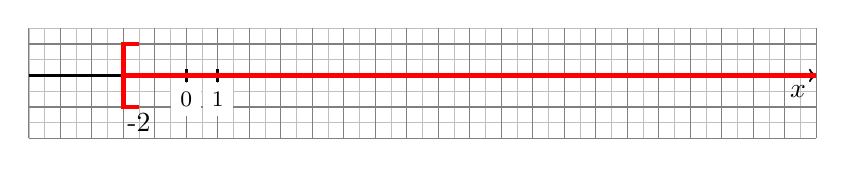
\begin{tikzpicture}[scale=0.4]
	\def\xY{-5};
	\def\yY{-2};
	\def\xZ{20};
	\def\yZ{1.5};
	\coordinate (Y) at (\xY,\yY);
	\coordinate (Z) at (\xZ,\yZ);
	\draw[step=0.5cm, lightgray, very thin] (Y) grid (Z);
	\draw[step=1cm, gray,thin] (Y) grid (Z);
	\draw[ ->,thick] (\xY, 0) -- (\xZ, 0) node[below left]{$x$};
	\foreach \x in {0,1}	\draw[very thick](\x,0.2cm)--(\x,-0.2cm) node[below,fill=white]{\footnotesize \x};
	\def\xbornea{-2};
	\def\orientationa{1};
	\draw[line width=1.7pt,red] ({\xbornea+0.5*\orientationa},1)--(\xbornea,1)--(\xbornea,-1)--({\xbornea+0.5*\orientationa},-1);
	\draw(\xbornea+0.5,-1.5)node{\xbornea};
	\def\xborneb{\xZ};
	\def\orientationb{1};
	\draw[line width=1.7pt,red](\xbornea,0)--(\xborneb,0);
	\end{tikzpicture}
	\end{center}
\end{ex}

\vspace{-5mm}
\begin{rmq}
Le symbole $\infty$ n'est pas un nombre réel. C'est pourquoi le crochet est toujours ouvert du côté de ce symbole.
\end{rmq}

\begin{exec}
\hspace{0.4cm} \hypertarget{Ex_3_2_1}{} \phantom{\ding{79}} Exercice \ref{3_2_1} \hspace{0.4cm};
\hspace{0.4cm} \hypertarget{Ex_3_2_2}{} \phantom{\ding{79}} Exercice \ref{3_2_2} \hspace{0.4cm};
\hspace{0.4cm} \hypertarget{Ex_3_2_3}{} \ding{79} Exercice \ref{3_2_3} \hspace{0.4cm}
\end{exec}

\section{Distance entre deux nombres réels}

\subsection{Notation $|a|$, $a \in \R$}

\begin{dft}
Soit $a$ un nombre réel.

\noindent On appelle valeur absolue de $a$, notée $|a|$, la distance entre $a$ et $0$
\end{dft}

\smallskip
\begin{ex}
Essayons de déterminer $|-12|$.\medskip 

\noindent On sait d'après la définition précédente que $|-12|$ est la \\distance entre $0$ et $-12$. On représente la droite des réels, \\puis (en rouge) la distance entre $0$ et $-12$ :

\vspace{-15mm}
\begin{flushright}
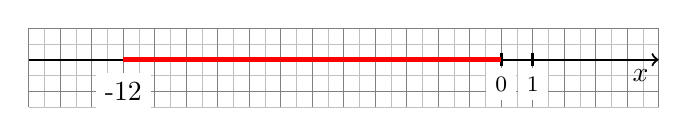
\begin{tikzpicture}[scale=0.4]
\def\xY{-15};
\def\yY{-1.5};
\def\xZ{5};
\def\yZ{1};
\coordinate (Y) at (\xY,\yY);
\coordinate (Z) at (\xZ,\yZ);
\draw[step=0.5cm, lightgray, very thin] (Y) grid (Z);
\draw[step=1cm, gray,thin] (Y) grid (Z);
\draw[ ->,thick] (\xY, 0) -- (\xZ, 0) node[below left]{$x$};
\foreach \x in {0,1}	\draw[very thick](\x,0.2cm)--(\x,-0.2cm) node[below,fill=white]{\footnotesize \x};
\def\xbornea{-12};
\def\orientationa{1};
\draw(\xbornea,-1)node[fill=white]{\xbornea};
\def\xborneb{0};
\def\orientationb{1};
\draw[line width=2pt,red](\xbornea,0)--(\xborneb,0);
\end{tikzpicture}
\end{flushright}

\noindent On remarque que, bien que $-12$ soit négatif, $|-12|$ est positif et est égale à $12$. En effet, $|-12|$ est une distance donc toujours positive.
\end{ex}

\begin{rmq}
Quelle que soit l'expression $a$, $a^2$ est toujours positive, donc $\sqrt{a^2}$ existe. Par exemple $\sqrt{3^2} = \sqrt{9} = 3$.

\noindent On peut donc en déduire une autre manière de définir la valeur absolue : \quad $|a| = \sqrt{a^2}$
\end{rmq}

\bigskip
\noindent Plus généralement, avec la notation valeur absolue, il est possible de définir la distance entre deux nombres réels :

\begin{prop}
Soient $a$ et $b$ deux nombres réels. $|a-b|$ ou $|b-a|$ est la distance entre $a$ et $b$ 
\end{prop}

\smallskip
\begin{ex}
Essayons de déterminer $|2-11|$.\medskip 

\noindent On sait d'après la définition précédente que $|2-11|$ est la \\distance entre $2$ et $11$. On représente la droite des réel, \\puis (en rouge) la distance entre $2$ et $11$ :
\\
\vspace{-19mm}
\begin{flushright}
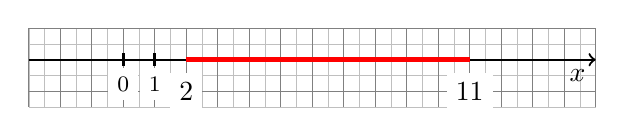
\begin{tikzpicture}[scale=0.4]
\def\xY{-3};
\def\yY{-1.5};
\def\xZ{15};
\def\yZ{1};
\coordinate (Y) at (\xY,\yY);
\coordinate (Z) at (\xZ,\yZ);
\draw[step=0.5cm, lightgray, very thin] (Y) grid (Z);
\draw[step=1cm, gray,thin] (Y) grid (Z);
\draw[ ->,thick] (\xY, 0) -- (\xZ, 0) node[below left]{$x$};
\foreach \x in {0,1}	\draw[very thick](\x,0.2cm)--(\x,-0.2cm) node[below,fill=white]{\footnotesize \x};
\def\xbornea{2};
\def\orientationa{1};
\draw(\xbornea,-1)node[fill=white]{\xbornea};
\def\xborneb{11};
\def\orientationb{1};
\draw(\xborneb,-1)node[fill=white]{\xborneb};
\draw[line width=2pt,red](\xbornea,0)--(\xborneb,0);
\end{tikzpicture}
\end{flushright}

\noindent La distance entre $2$ et $11$ vaut $9$. Donc $|2-11| = 9$
\end{ex}

\subsection{Notion d'intervalle centré}

\begin{dft}
Soient $a$ un nombre réel et $r$ un nombre réel positif. 

\noindent L'intervalle \quad $[a-r;a+r]$ \quad est un intervalle centré en \quad $a$ \quad de longueur \quad $2r$.
\end{dft}

\smallskip
\begin{ex}
Essayons de représenter l'intervalle pour $a=7$ et $r=10$ soit l'intervalle $[7-10;7+10]$.\medskip 

\noindent On représente la droite des réels, \\puis (en violet) la valeur $7$ :

\vspace{-12mm}
\begin{flushright}
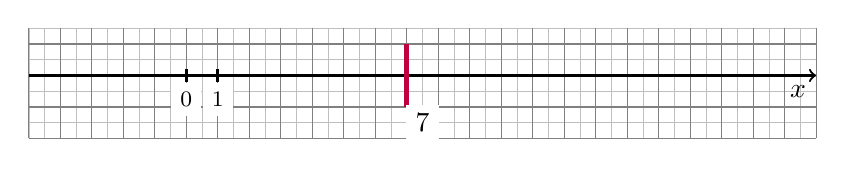
\begin{tikzpicture}[scale=0.4]
\def\xY{-5};
\def\yY{-2};
\def\xZ{20};
\def\yZ{1.5};
\coordinate (Y) at (\xY,\yY);
\coordinate (Z) at (\xZ,\yZ);
\draw[step=0.5cm, lightgray, very thin] (Y) grid (Z);
\draw[step=1cm, gray,thin] (Y) grid (Z);
\draw[ ->,thick] (\xY, 0) -- (\xZ, 0) node[below left]{$x$};
\foreach \x in {0,1}	\draw[very thick](\x,0.2cm)--(\x,-0.2cm) node[below,fill=white]{\footnotesize \x};
\def\xbornea{7};
\def\orientationa{1};
\draw[line width=1.7pt,purple] (\xbornea,1)--(\xbornea,-1);
\draw(\xbornea+0.5,-1.5)node[fill=white]{\xbornea};
\end{tikzpicture}
\end{flushright}


\noindent On représente, en bleu, les valeurs comprises \\dans l'intervalle $[7-10;7]$ et, en rouge, les \\valeurs comprises dans l'intervalle $[7;7+10]$.

\vspace{-18mm}
\begin{flushright}
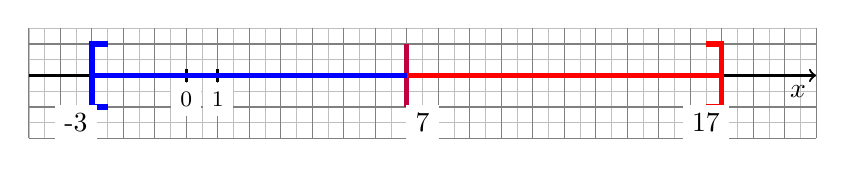
\begin{tikzpicture}[scale=0.4]
\def\xY{-5};
\def\yY{-2};
\def\xZ{20};
\def\yZ{1.5};
\coordinate (Y) at (\xY,\yY);
\coordinate (Z) at (\xZ,\yZ);\draw[step=0.5cm, lightgray, very thin] (Y) grid (Z);
\draw[step=1cm, gray,thin] (Y) grid (Z);
\draw[ ->,thick] (\xY, 0) -- (\xZ, 0) node[below left]{$x$};
\foreach \x in {0,1}	\draw[very thick](\x,0.2cm)--(\x,-0.2cm) node[below,fill=white]{\footnotesize \x};
\def\xbornea{7};
\def\orientationa{1};
\draw[line width=2pt,purple] (\xbornea,1)--(\xbornea,-1);
\draw(\xbornea+0.5,-1.5)node[fill=white]{\xbornea};
\def\xborneb{17};
\def\orientationb{1};
\draw[line width=2pt,red] ({\xborneb-0.5*\orientationb},1)--(\xborneb,1)--(\xborneb,-1)--({\xborneb-0.5*\orientationb},-1);
\draw(\xborneb-0.5,-1.5)node[fill=white]{\xborneb};
\draw[line width=2pt,red](\xbornea,0)--(\xborneb,0);
\def\xbornec{-3};
\def\orientationc{-1};
\draw[line width=2pt,blue] ({\xbornec-0.5*\orientationc},1)--(\xbornec,1)--(\xbornec,-1)--({\xbornec-0.5*\orientationc},-1);
\draw(\xbornec-0.5,-1.5)node[fill=white]{\xbornec};
\draw[line width=2pt,blue](\xbornea,0)--(\xbornec,0);
\end{tikzpicture}
\end{flushright}

\end{ex}

\medskip
Sur l'exemple précédent, on remarque que la distance entre la borne minimale, ici $-3$, et $7$ est la même que la distance entre la borne maximale de l'intervalle, ici $17$, et $7$.

\noindent Cet intervalle est donc centré en $7$ et la distance entre le centre de l'intervalle et une borne est toujours inférieure ou égale à $10$. On peut donc définir ce genre d'intervalle grâce à la valeur absolue :

\begin{prop}
Soient $a$ un nombre réel et $r$ un nombre réel positif.

\noindent L'intervalle \quad $[a-r;a+r]$ \quad peut être caractérisé par la condition :  \begin{center}
Pour tout $x \in \R$, $|x-a| \leqslant r$
\end{center}
\end{prop}

\end{document}